\section{Proposed System Architecture}

\subsection{Formal Problem Formulation}
Let $\mathcal{D}$ denote the universe of recruitment documents partitioned into job descriptions $\mathcal{J}$ and candidate resumes $\mathcal{C}$. Given a query document $D_q \in \mathcal{D}$ and candidate corpus $\mathcal{C}_{cand} = \{D_1, D_2, \dots, D_N\}$, the objective of bidirectional matching is to compute a ranking permutation $\pi$ over $\mathcal{C}_{cand}$ that maximizes ranking relevance ($nDCG@K$) with respect to ground-truth relevance grades $\mathbf{y}_q \in \{0, 1, 2, 3\}^N$:
\begin{equation}
    \pi^* = \arg\max_{\pi} \text{nDCG}@K\big( \pi(\mathcal{C}_{cand}), \mathbf{y}_q \big).
\end{equation}

\begin{figure}[t]
\centering
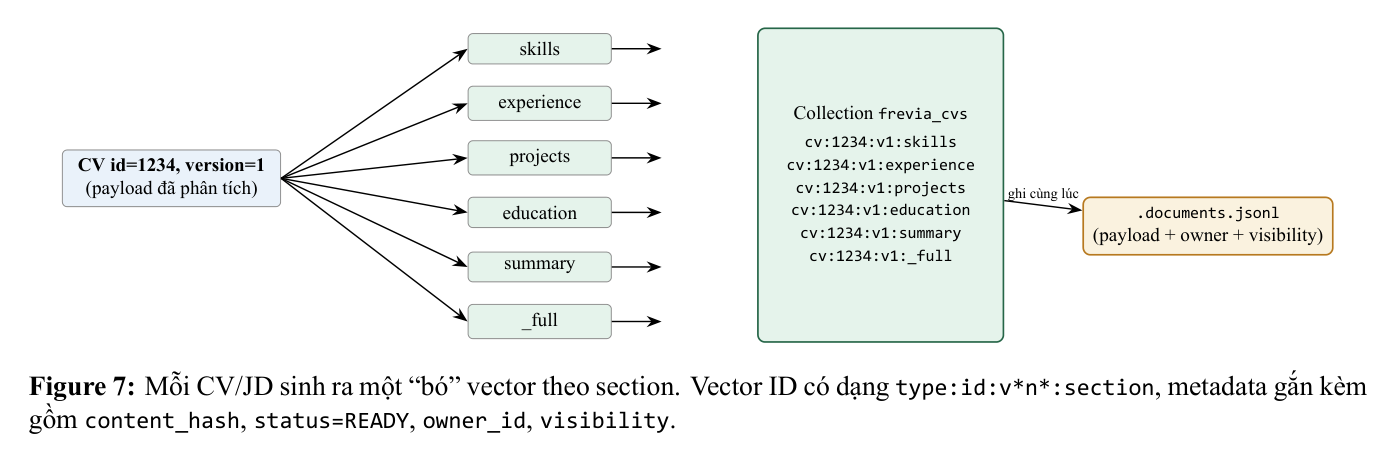
\includegraphics[width=0.88\textwidth]{figures/fig07_vector_theo_section.png}
\caption{Section-aware multi-vector representation and alignment between Job Description (JD) and Curriculum Vitae (CV).}
\label{fig:arch}
\end{figure}

The architecture decouples processing into two operational pipelines:
\begin{itemize}
    \item \textbf{Offline Pipeline (Indexing \& Sync)}: Extracts canonical metadata, segments raw text into functional sections via rule-based boundary detection, generates frozen dense representations, and updates ChromaDB indexes asynchronously.
    \item \textbf{Online Pipeline (Serving \& Explanation)}: Executes two-stage candidate retrieval, computes cross-section similarity matrices, applies hybrid constraint fusion, and generates evidence-grounded justifications on demand.
\end{itemize}

\subsection{Section Decomposition and Multi-Vector Representation}
Given document $D$, the parser segments raw text into $M$ functional sections using heading boundary patterns:
\begin{equation}
    D = \Big\{ \big(s_1, T_1\big), \big(s_2, T_2\big), \dots, \big(s_M, T_M\big), \big(\text{full}, T_{raw}\big) \Big\},
\end{equation}
where $s_m \in \{\text{skills}, \text{experience}, \text{education}, \text{summary}, \text{projects}\}$. Each section text $T_m$ as well as full text $T_{raw}$ is mapped into a $d$-dimensional vector space via a frozen bi-encoder $\mathcal{E}(\cdot)$:
\begin{equation}
    \mathbf{v}_m = \mathcal{E}(T_m) \in \mathbb{R}^d, \quad \mathbf{v}_{full} = \mathcal{E}(T_{raw}) \in \mathbb{R}^d, \quad \|\mathbf{v}\|_2 = 1.
\end{equation}

\subsection{Section Matching and Dynamic Renormalization}
For query $D_q$ and candidate $D_c$, section similarity uses cosine metric:
\begin{equation}
    \text{sim}(\mathbf{u}, \mathbf{w}) = \frac{\mathbf{u} \cdot \mathbf{w}}{\|\mathbf{u}\|_2 \|\mathbf{w}\|_2}.
\end{equation}
To accommodate non-standard document structures where technical proficiencies are described in narrative work history rather than dedicated skill sections, we employ \textbf{Cross-Section Pairing}:
\begin{equation}
    c(s_m) = \max_{s_k \in D_c} \text{sim}\big(\mathbf{v}_q^{s_m}, \mathbf{v}_c^{s_k}\big).
\end{equation}

When documents omit optional sections (\textit{e.g.}, junior profiles lacking formal project portfolios, or freelance JDs lacking degree requirements), applying fixed zero-imputation would penalize valid candidates unfairly. We resolve this via \textbf{Dynamic Weight Renormalization}:
\begin{equation}
    S_{sem} = \frac{\sum_{m \in \mathcal{S}_{\text{matched}}} w_m \cdot c(s_m)}{\sum_{m \in \mathcal{S}_{\text{matched}}} w_m},
\end{equation}
where $\mathcal{S}_{\text{matched}}$ is restricted strictly to active query sections, calibrated with baseline domain weights ($w_{\text{skills}} = 0.35, w_{\text{exp}} = 0.35, w_{\text{proj}} = 0.15, w_{\text{edu}} = 0.10, w_{\text{sum}} = 0.05$).

\subsection{Hybrid Ranking Engine: Two-Tier Separation}
\label{sec:hybrid}
To preserve clear semantics, the system enforces a strict two-tier separation between \textit{eligibility constraints} and \textit{competency ranking}:
\begin{itemize}
    \item \textbf{Tier 1: Eligibility Hard Filters}: Candidates are pre-filtered based on non-competency market boundaries (active account status, public privacy permissions, task availability, and budget upper-bound constraints).
    \item \textbf{Tier 2: Competency Ranking}: Surviving candidates are scored via unified hybrid fusion:
    \begin{equation}
        S_{hybrid} = \alpha \cdot S_{sem} + (1 - \alpha) \cdot \big[ w_{skl} S_{skills} + w_{exp} S_{exp} + w_{pref} S_{pref} \big].
        \label{eq:hybrid}
    \end{equation}
\end{itemize}

\textbf{Asymmetric Skill Coverage vs. Symmetric Jaccard}: Rather than penalizing qualified candidates who possess auxiliary skills beyond the job specification, $S_{skills}$ evaluates asymmetric requirement recall over normalized skill aliases:
\begin{equation}
    \text{Cov}(\mathcal{T}) = \frac{\sum_{t \in \mathcal{T}} \mathbb{I}(t \in \mathcal{C}_{skills}) \cdot w_t}{\sum_{t \in \mathcal{T}} w_t}, \quad S_{skills} = 0.8 \cdot \text{Cov}(\text{MustHave}) + 0.2 \cdot \text{Cov}(\text{NiceToHave}).
\end{equation}
When candidates lack more than $50\%$ of mandatory must-have skills, a multiplicative penalty factor $\gamma = \text{Cov}(\text{MustHave})$ is applied to prevent compensation by non-essential criteria.

\subsection{Architectural Decisions and Empirical Rationales}
Table~\ref{tab:design_decisions} summarizes the architectural choices governing the pipeline.

% Auto-generated: Design Decisions, Rationales, and Empirical Evidence
\begin{table*}[t]
\centering\small
\caption{System Design Decisions, Alternatives Considered, Architectural Rationales, and Empirical Evidence.}
\label{tab:design_decisions}
\resizebox{\textwidth}{!}{%
\begin{tabular}{@{}llll@{}}
\toprule
\textbf{Design Decision} & \textbf{Alternative Considered} & \textbf{Architectural Rationale} & \textbf{Empirical Evidence} \\ \midrule
\textbf{Multi-Vector Sectioning} & Flat Single-Vector / Chunking & Prevents semantic dilution of sparse technical skills & $+25.6\%$ nDCG@10 over single-vector ($p < 0.001$) \\
\textbf{Cross-Section Pairing} & Fixed Same-Name Matching & Maps skills embedded inside experience/project text & $+2.7\%$ nDCG@10 over fixed; $26\%$ CVs lack dedicated skill header \\
\textbf{Dynamic Renormalization} & Zero-Imputation & Prevents penalizing junior CVs lacking optional sections & Preserves score calibration when sections are omitted \\
\textbf{Skill Coverage Scoring} & Symmetric Jaccard & Evaluates requirement recall without penalizing auxiliary skills & Ablation shows $S_{skills}$ is vital ($-26.13\%$ drop when omitted) \\
\textbf{Two-Stage Retrieval ($K=100$)} & Full Brute-Force Scanning & Retains $>85\%$ coarse recall while ensuring sub-30\,ms latency & $14.25\times$ speedup at $N=5,000$ candidates ($25.2$\,ms vs. $360.1$\,ms) \\
\textbf{Grounded Explanation} & End-to-End Generative LLM & Generates claims directly from score breakdown & $95.41\%$ verbatim groundedness; $4.59\%$ hallucination rate \\ \bottomrule
\end{tabular}%
}
\end{table*}


